\documentclass[a4paper, 11pt,titlepage, openright, twoside]{report}
\usepackage[utf8]{inputenc}
\usepackage[T1]{fontenc}
\usepackage{silence}
\usepackage{amsmath,amsfonts,amssymb,amsthm}
\usepackage{mathtools}
\usepackage[inline]{enumitem}
\usepackage{newunicodechar}
\usepackage[margin=3cm,bindingoffset=1cm]{geometry}
\usepackage{stmaryrd}
\SetSymbolFont{stmry}{bold}{U}{stmry}{m}{n}
% https://tex.stackexchange.com/a/106719
\DeclareSymbolFont{sfletters}{OML}{cmbrm}{m}{it}
\usepackage[nopatch=footnote]{microtype}
\usepackage[dvipsnames]{xcolor}
\usepackage{mathpartir}
\usepackage{biblatex}
\usepackage{hyperref}
\usepackage{cleveref}
\usepackage{tikz}
\usepackage{tikz-cd}
\usepackage{listings}
\lstset{basicstyle= \footnotesize \ttfamily}
\lstset{language=ml}

\usepackage[nodisplayskipstretch]{setspace}
\setlength{\parskip}{0pt}

\addbibresource{refs.bib}


\title{\textbf{A Fine Calculus for Static Delimited Control}}
\author{Wiktor Kuchta}

\date{60 września 2024} %TODO

\usepackage{titling}

\renewcommand \maketitlehookb {
  \begin{center}\large
  Fajny rachunek dla statycznie ograniczonych operatorów sterowania
  \end{center}
  \vfil
}

\renewcommand \maketitlehookc {
  \vfil
  \begin{center}
  \large Praca magisterska \\[0.85em]
  \begin{tabular}[t]{rl}
  \textbf{Promotor:} & dr hab. Dariusz Biernacki
  \end{tabular}\end{center}
  \vfil\vfil\vfil\vfil
  \begin{center}Uniwersytet Wroc\l{}awski\\
  Wydzia\l{} Matematyki i Informatyki\\
  Instytut Informatyki
  \end{center}
}


\newcommand{\shiftz}{\textsf{shift0}}
\newcommand{\keyword}[1]{\textsf{\textup{#1}}}
\newcommand{\KwOp}{\keyword{op}}
\newcommand{\Op}{\KwOp\,}
\newcommand{\KwHandle}{\keyword{handle}}
\newcommand{\Handle}{\KwHandle\;}
\newcommand{\KwWith}{\keyword{with}}
\newcommand{\With}{\;\KwWith\;}
\newcommand{\KwRaise}{\keyword{raise}}
\newcommand{\Raise}{\KwRaise\;}
\newcommand{\KwTry}{\keyword{try}}
\newcommand{\Try}{\KwTry\;}
\newcommand{\KwLet}{\keyword{let}}
\newcommand{\Let}[3]{\keyword{let}\;#1\;\keyword{=}\;#2\;\keyword{in}\;#3}
\newcommand{\RLet}[3]{\Let{#1}{\raisebox{0.5 ex}{$#2$}}{#3}}
\newcommand{\KwLift}{\keyword{lift}}
\newcommand{\Lift}[1]{\KwLift\;#1}
\newcommand{\subst}[2]{\{#1{:=}#2\}}
\newcommand{\E}{\mathcal{E}}
\newcommand{\K}{\mathcal{K}}
\renewcommand{\S}{\mathcal{S}}
\newcommand{\A}{\mathcal{A}}
\newcommand{\kT}{\mathsf{T}}
\newcommand{\kE}{\mathsf{E}}
\newcommand{\kR}{\mathsf{R}}
\newcommand{\Free}{\textrm{-}\mathrm{free}}
\newcommand{\Obs}{\mathrm{Obs}}
\newcommand{\N}{\mathbb{N}}
\DeclareMathOperator{\dom}{dom}
\newcommand{\+}{\enspace}
\newcommand{\lStr}{\textsf{Str}}
\newcommand{\lPar}{\textsf{Par}}

\newtheorem{corollary}{Corollary}
\newtheorem{lemma}{Lemma}
\newtheorem{theorem}{Theorem}
\newtheorem{prop}{Proposition}


\newunicodechar{│}{\mid} % Digr vv
\newunicodechar{╱}{\mathbin{/}} % Digr FD
\newunicodechar{∷}{::} % Digr ::
\newunicodechar{□}{\square} % Digr OS
\newunicodechar{∅}{\emptyset} % Digr /0
\newunicodechar{α}{\alpha}
\newunicodechar{β}{\beta}
\newunicodechar{δ}{\delta} % Digr d*
\newunicodechar{ε}{\varepsilon}
\newunicodechar{γ}{\gamma} % Digr g*
\newunicodechar{ι}{\iota} % Digr i*
\newunicodechar{κ}{\kappa}
\newunicodechar{λ}{\lambda}
\newunicodechar{μ}{\mu}
\newunicodechar{ν}{\nu}
\newunicodechar{ρ}{\rho}
\newunicodechar{σ}{\sigma}
\newunicodechar{τ}{\tau}
\newunicodechar{η}{\eta} % Digr y*
\newunicodechar{Δ}{\Delta}
\newunicodechar{Γ}{\Gamma}
\newunicodechar{Ω}{\Omega} % digr W*
\newunicodechar{ℕ}{\N} % Digr NN 8469 nonstandard
\newunicodechar{⊆}{\subseteq} % Digr (_
\newunicodechar{∪}{\cup} % Digr )U
\newunicodechar{∈}{\in} % Digr (-
\newunicodechar{∃}{\exists} % Digr TE
\newunicodechar{∀}{\forall} % Digr FA
\newunicodechar{∧}{\wedge} % Digr AN
\newunicodechar{∨}{\vee} % Digr OR
\newunicodechar{⊥}{\bot} % Digr -T
\newunicodechar{⊢}{\vdash} % Digr \- 8866 nonstandard
\newunicodechar{⊨}{\models} % Digr \= 8872 nonstandard
\newunicodechar{⊤}{\top} % Digr TO 8868 nonstandard
\newunicodechar{⇒}{\implies} % Digr =>
\newunicodechar{⇔}{\iff} % Digr ==
\newunicodechar{↦}{\mapsto} % Digr T> 8614 nonstandard
\newunicodechar{≠}{\neq}
\newunicodechar{⟦}{\llbracket} % Digr [[ 10214 nonstandard (needs pkg stmaryrd)
\newunicodechar{⟧}{\rrbracket} % Digr ]] 10215 nonstandard
\newunicodechar{≥}{\ge}
\newunicodechar{≤}{\le}
\newunicodechar{≡}{\equiv}
\newunicodechar{≈}{\approx}


% cursed
\WarningFilter{newunicodechar}{Redefining Unicode}
\newunicodechar{·}{\ifmmode\cdot\else\textperiodcentered\fi} % Digr .M
\newunicodechar{×}{\ifmmode\times\else\texttimes\fi} % Digr *X
\newunicodechar{→}{\ifmmode\rightarrow\else\textrightarrow\fi} % Digr ->
\newunicodechar{←}{\ifmmode\leftarrow\else\textleftarrow\fi} % Digr <-
\newunicodechar{…}{\ifmmode\dots\else\textellipsis\fi} % Digr .,
\newunicodechar{⟨}{\langle}
\newunicodechar{⟩}{\rangle}

\begin{document}

\maketitle


\thispagestyle{empty}
\cleardoublepage
\begin{abstract}
	We consider a variant of the call-by-value $λμ$-calculus extended with control delimiters,
	in which $μ$ becomes the static delimited control operator shift0.
	We propose new reduction rules for cases where the captured continuation can be determined statically.
	We prove the calculus confluent and adequate wrt.\,operational semantics.
	We then let delimiters carry data (resulting in a form of dynamic binding), which lets us express deep effect handlers.
	The new reductions cooperate with the encoding to let us statically handle effects.
	We also propose natural encodings of return clauses for delimiters.
%	We propose purity assertions for lightweight purity-based reasoning.
%	We prove the reduction is confluent and adequate wrt.\ operational semantics.
	We argue that the calculus is stronger than previous results in the literature and could form basis for
	reasoning and optimizations for the aforementioned forms of control.
	\begin{center} \rule[3pt]{300pt}{1pt} \end{center}
	polski
\end{abstract}


\thispagestyle{empty}
\cleardoublepage
\setcounter{page}{5}
\tableofcontents


\chapter{Introduction}
Consider a program of the following form in a language with (unnamed) exceptions:
\begin{align*}
	&\Try \\
	&\quad \Let{x}{e}{\Raise (x*2)} \\
	&\KwWith\; z.\,z*3
\end{align*}
If the execution gets to $\Raise (x*2)$, the handler will catch the exception and produce the result $x*2*3$.
%$$\Try \Let{x}{e}{\Raise (2*x)} \With z.\,3 * z$$
%We know that \textit{the} $\KwRaise$ (if we get to it) is going to be handled by \textit{the} handler.
%And in that case, $x*2$ is going to be multiplied by $3$.
How to \textit{optimize} the program, so that we only perform one multiplication, $x*6$?

We can ask a similar question for \textit{effect handlers}.
This generalization allows us to capture the \textit{continuation} of the \textit{operation} (a.k.a.\,\textit{generic effect}) we are handling
and bind it as a variable.
The conventional evaluation step rule is
$$\Handle E[\Op v] \With x\;k.\,e ↦  e\subst{x}{v}\subst{k}{λy.\,\Handle E[y] \With x\;k.\,e} $$
This is a form of \textit{static delimited control}: control because we capture continuations,
delimited because the continuation is delimited by the handler, and static because the delimiter remains
in the captured continuation.
%The last part is crucial.

Let's consider a similar example:
$$ \Handle \Let{x}{e}{\Op (x*2)} \With z\;k.\,k\,(z*3) $$
Similarly to the example of exceptions, we know that $\Op (x*2)$ will be handled
by the $z\;k.\,k\,(z*3)$ handler -- even if the evaluation of $e$ captures continuations,
the $\KwOp$ and $\KwHandle$ will stay together.
%Now let's argue semi-formally why the handler will handle the operation.% (if we get to it).
%%Let's assume $e$ doesn't loop forever, otherwise we don't get to it.
%\begin{enumerate}
%	\item
%	If $e$ evaluates to a value $v$,
%	% (which is necessary to reach the $\KwRaise$)
%	then by the rule $\Let{x}{v}{t} ↦ t\subst{x}{v}$ we get
%	$$ \Handle {\Op (v*2)} \With z\;k.\,k\,(z*3) $$
%	and the previous rule applies.
%	%$$ (λy.\,\Handle y \With z\;k.\,k\,(z*3)) ((v*2)*3)$$
%	%If $e$ installs any handlers, their scope is limited to remain inside $e$, and won't influence the $\KwRaise$.
%	\item
%	If $e$ performs an operation and doesn't handle it internally, then the captured continuation will be
%	$λy.\,\Handle \Let{x}{E[y]}{\Op (x*2)} \With z\;k.\,k\,(z*3)$.
%	The body of the abstraction is the expression we originally considered but after some evaluation steps, so we reason by induction.
%\end{enumerate}

We therefore know the substitution that will be performed during the handling of the operation:
$z:=x*2$. Exactly this substitution is needed to rewrite the two multiplications into one.
We even know that $k:=λy.\,\Handle y \With z\;k.\,k\,(z*3)$.
But we can't substitute that into the clause, because the clause is shared for all operations inside,
and $x$ is not even in scope.

What we can do is copy the clause, perform the substitution and \textit{abort} the handler:
$$\Handle \Let{x}{e}{\A\,(k (z*3))\subst{z}{x*2}\subst{k}{λy.\,\Handle \Let{x}{e}}}$$

So let's instead consider the other form of static delimited control, $\shiftz$ and $\textsf{reset}$,
which is closely related to deep effect handlers. The evaluation rule is:
$$⟨E[\shiftz\,k.\,e]⟩ ↦ e\subst{k}{λy.\,⟨E[y]⟩}$$
Here, \textsf{reset} (written $⟨·⟩$) is the delimiter and doesn't have any clauses.
Instead, the body of the $\shiftz$ tells us what to do with the captured continuation.
The final form of our example is
$$\Let{op}{λz.\,x*2}⟨\Let{x}{e}{\shiftz\,k.\,k\,(z*3)}$$
And finally, we have our reduction rule:
$$⟨L[E[\shiftz\,k.\,e]]⟩ → ⟨L[\A\,e\subst{k}{λy.\,⟨E[y]⟩}]⟩$$

If that problem 

\begin{enumerate}
	\item
		We introduce an extension of the $λμ$-calculus with delimiters, where
		$μ$ behaves like the $shift0$ operator
	\item
		We add new reduction rules that let us statically determine the captured continuation.
	\item
		We prove the above rules confluent and adequate wrt.\,operational semantics
	\item
		We let delimiters carry data
\end{enumerate}


We haven't figured out a rewrite rule for our optimization yet.
The key part that allows it is the substitution for $z$ and $k$






It should be intuitively clear that the $\KwRaise$ we see is going to be handled by the exception handler we see.
That is, if we get to it at all, since $e$ might loop forever or exit the program or crash or raise an exception.
It might install a handler of its own, but it won't contain $\Raise Exn$ in scope, so it doesn't affect it.
If all of that didn't happen and $e_1$ happily evaluated to a value $n$, then we can perform an evaluation step
and get
$$\Try \Raise (2*n) \With z → 1+z$$
At this point, we can refer to the evaluation rule for handling a raised exception
$$\Try E[\Raise v] \With z → e_h ↦  e_h\subst{z}{v}$$
where $E$ are contexts of the form $E ::= □ │ \Let{x}{E}{e}$.
Applying this to our example, we get $3*(2*n)$, which we could simplify to $6*n$.

Shouldn't we be able to \textit{optimize} the program to get from two multiplications to just one?
Of course, this is a very basic and contrived example.
But optimization is often about many almost trivial steps that in the end
amount to big improvements.

Generalizing the above example, we can say that for a program of the form $\Try L[E[\Raise v]] \With z. e$
where $L$ are sequences of $\KwLet$s, i.e. $L ::= □ │ \Let{x}{e}{L}$,
if we get to executing the $\KwRaise$, then $e\subst{z}{v}$ will be the result.
How to turn this insight into a rewrite rule?

We can't perform the substitution in the handler's clause, since we are focusing
on one $\KwRaise$ and there might be potential previous $\KwRaise$s inside $L$.
It wouldn't make sense anyway since $v$ might refer to variables bound in $L$.
We have to rewrite the $\Raise v$. We consider a new construct $\A\, e$ that \textit{aborts}
the exception handler, ignoring its clauses and returns the result $e$.
The rewrite rule is
$$\Try L[E[\Raise v]] \With z.\, e  → \Try L[\A\,e\subst{z}{v}] \With z.\,e$$
We copy the handler clause to the place of the $\KwRaise$, apply the substitution,
and perform the abort $\A$ which bypasses the usual flow of exception handling.

Applying it to our original example, we get
$$\Try \Let{x}{e}{\A\,(3*(2*x))}\With z.\,3*z$$
in which we can perform our desired rewrite $3*(2*n) → 6*n$.

All of the above extends to \textit{effect handlers}.
Effect handlers are exception handlers, where the clause can also refer to the \textit{continuation}:
$$\Try E[\Raise v] \With z\;k.\, e → e\subst{z}{v}\subst{k}{λx.\,\Try E[x] \With z\;k.\,e}$$
This is a powerful feature that lets us write code with effectful operations,
whose interpretations can be dynamically provided by the handlers.




\chapter{Syntax}



\chapter{Confluence}

\section*{The problems with $\KwLet$ reassociation}

The $\KwLet$ reassociation reduction
$$\RLet{x}{\Let{y}{e}{t_1}}{t_2} → \Let{y}{e}{\Let{x}{t_1}{t_2}}$$
flattens the structure of the term by getting rid of $\KwLet$s nested on the left
(here raised).
It has the following critical pair with itself:
$$
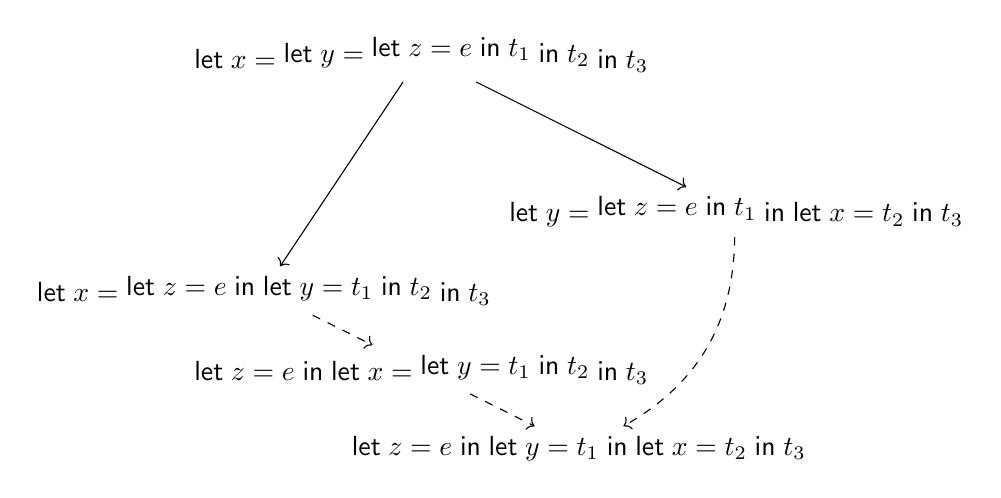
\begin{tikzpicture}
	\node (E1) at (2,5) {$\RLet{x}{\RLet{y}{\Let{z}{e}{t_1}}{t_2}}{t_3}$};
	\node (E2) at (6,3) {$\RLet{y}{\Let{z}{e}{t_1}}{\Let{x}{t_2}{t_3}}$};
	\node (E3) at (0,2) {$\RLet{x}{\Let{z}{e}{\Let{y}{t_1}{t_2}}}{t_3}$};
	\node (E3') at (2,1) {$\Let{z}{e}{\RLet{x}{\Let{y}{t_1}{t_2}}}{t_3}$};
	\node (E4) at (4,0) {$\Let{z}{e}{\Let{y}{t_1}{\Let{x}{t_2}{t_3}}}$};
	\path[->]
		(E1) edge (E2)
		(E1) edge (E3);
	\path[->,dashed]
		(E2) edge[bend left] (E4)
		(E3) edge (E3')
		(E3') edge (E4);
	%\draw [brown] (current bounding box.south west) rectangle (current bounding box.north east);
\end{tikzpicture}
$$
Two steps are needed on the left to complete the diagram.
This calls for the following generalization, which can do it in one step and \textit{does} have the diamond property:
$$\Let{x}{L[t_1]}{t_2} → L[\Let{x}{t_1}{t_2}]$$
However, this is not enough for \textit{parallel} reduction.
Here, the redex above overlaps with two different redexes below:
$$
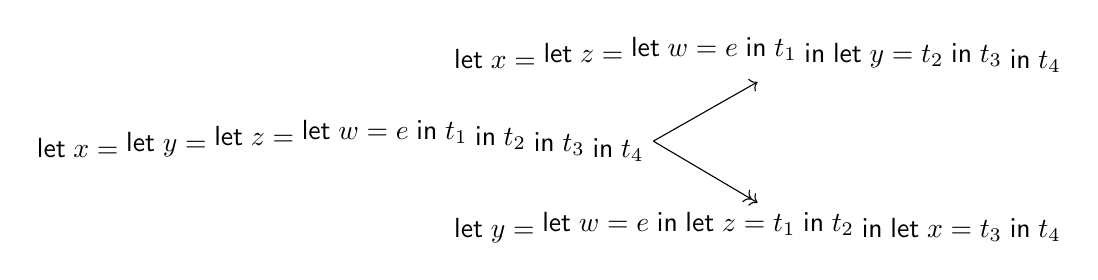
\begin{tikzpicture}
	\node (E1) at (0,0) {$\RLet{x}{\RLet{y}{\RLet{z}{\Let{w}{e}{t_1}}{t_2}}{t_3}}{t_4}$};
	\node (E2) at (5.3,1.1) {$\RLet{x}{\RLet{z}{\Let{w}{e}{t_1}}{\Let{y}{t_2}}{t_3}}{t_4}$};
	\node (E3) at (5.3,-1.1) {$\RLet{y}{\Let{w}{e}{\Let{z}{t_1}}{t_2}}{\Let{x}{t_3}}{t_4}$};
	\path[->] (E1.east) edge[] (E2.south);
	\path[->>] (E1.east) edge[] (E3.north);
	%\draw [brown] (current bounding box.south west) rectangle (current bounding box.north east);
\end{tikzpicture}
$$
To complete this diagram in one parallel reduction step, it would need to have not only length-wise, but also a depth-wise generalization
of $\KwLet$ reassociation.
We don't provide a definition here, since we haven't managed to prove any attempt right.

The other challenge is that a $let.\S$ reduction can tear apart a $let.let$ redex:
$$
\begin{tikzpicture}
	\node (E1) at (0,0) {$\Let{x}{\Let{y}{\S κ.\,e}{t_1}}{t_2}$};
	\node (E2) at (3.5,-2) {$\Let{y}{\S κ.\,e}{\Let{x}{t_1}{t_2}}$};
	\node (E3) at (-3.5,-1.333) {$\Let{x}{\S κ.\,e\subst{κ}{κ[\Let{y}{□}{t_1}]}}{t_2}$};
	\node (E3') at (-3.5,-2.666) {$\S κ.\,e\subst{κ}{κ[\Let{x}{\Let{y}{□}{t_1}}{t_2}]}$};
	\node (E4) at (0,-4) {$\S κ.\,e\subst{κ}{κ[\Let{y}{□}{\Let{x}{t_1}{t_2}}]}$};
	\path[->] (E1) edge (E2);
	\path[->] (E1) edge (E3);
	\path[->,dashed] (E3) edge (E3') (E2) edge (E4);
	\path[->>,dashed] (E3') edge (E4);
\end{tikzpicture}
$$
We need a successive $let.\S$ step to make the $let.let$ redexes whole, now after structural substitution.


Let's demonstrate the main challenges for proving confluence.
Previous proofs of confluence for $λμ$-calculi amounted to the diamond property of parallel reduction.
The problem with confluence is that structural reduction ($let.\S$) can tear redexes apart, as in:
$$\Let{x}{\Let{y}{\S κ.\,e}{t_1}}{t_2}$$
$$⟨L[\Let{x}{\S κ.\,e}{\S κ.\,t}]⟩$$
and additional structural reductions are needed to make the $let.let$%
%\footnote{
%	Herbelin and Zimmerman \cite{Herbelin} report no problems with the critical pair involving $let.\S$ and $let.let$.
%	$let.let$ by itself poses problems, with 
%	We believe that's because they used a rule $κ[\Let{x}{e}{t}] → \Let{x}{e}{κ[t]}$, which seems to be valid in the undelimited case.
%	This rule doesn't figure in the paper, but a similar one $z(\Let{x}{e}{t}) → \Let{x}{e}{zt}$ does.
%}
and $dlets.\S$ redexes whole again,
now inside $e$.
Conversely, the structural substitution can push the $k.\S$ redex apart:
$$κ[\S κ'.\,e]\subst{κ}{κ[\Let{x}{□}{t}]} = κ[\Let{x}{\S κ'.\,e}{t}]$$
Therefore a parallel reduction involving the entirety of the calculus needs to be generalized to involve multiple structural reduction steps in some places.
Naively, such a definition would need to recursively refer to a parallel reduction of a term \textit{after} structural substitution.
Such a term may be bigger than the original, which poses problems for inductive proofs.

The parallel reduction approach does work, however, for the subcalculus without $let.let$ and without delimiters carrying data.

We will prove confluence of $\xrightarrow{\lStr} ∪ \Rrightarrow$,
where $\xrightarrow{\lStr}$ are structural reductions and $\Rrightarrow$ is a parallel reduction
containing the other reductions,
by the method of decreasing diagrams \cite{dd}.
Confluence of $→$ will follow from ${→} ⊆ {\xrightarrow{Str} ∪ \Rrightarrow} ⊆ {→^*}$.

We label $e \xrightarrow{\lStr} e'$ by $(\lStr, e)$ and $e \Rrightarrow e'$ by $\lPar$ and order the labels thus:
for all $e$ set $\lPar > (\lStr, e)$ and for all $e, e'$ set $(\lStr, e) > (\lStr, e')$ iff $e \xrightarrow{\lStr}\mathrel{\vphantom{\to}^+} e'$.
We need to prove that the order on labels is well-founded and that we can complete the three kinds of local peaks
into decreasing valleys.\footnote{
	The proof scheme is essentially Exercise 14.2.25 in Terese \cite{Terese}.
}

\section*{Strong normalization of $\xrightarrow{Str}$}
Well-foundedness of the labels will follow from strong normalization of
$$\xrightarrow{Str} \;=\; \xrightarrow{let.\S} ∪ \xrightarrow{d.\S} ∪ \xrightarrow{k.\S}.$$
We adapt the approach of de Groote\cite{Groote}.

and the ``frame occurences''\footnote{
	We count the continuation frame before ($1$) and after the potential capture by a $\S κ.\, e$ ($\#_κ e$).
} $\#$ and ``continuation variable count'' $\#_κ$ as follows:
\begin{align*}
	\# X[\S κ. e] &= 1 + \#_κ e \\
	\# e &= 1 \text{ otherwise} \\
%	\\
	\#_κ x &= 0 \\
	\#_κ λx. e &= \#_κ e \\
	\#_κ \S κ'.\,e &= \#_κ e \\
	\#_κ v\;u &= \#_κ v + \#_κ u \\
	\#_κ \Let{x}{e}{t} &= \#_κ e + \# e · \#_κ t \\
	\#_κ ⟨e⟩ &= \#_κ e \\
	\#_κ κ[e] &= \#_κ e + \# e \\
	\#_κ κ'[e] &= \#_κ e
\end{align*}
where $X$ are ``free contexts'' that skip across $\S$-delimiter brackets:
$$X ::= □ │ \Let{x}{X}{t} │ ⟨X[\S κ.\,X]⟩ │ κ[X[\S κ'.\,X]]$$
The idea is a $\KwLet$ can be captured by a particular $\S$
iff the term can be written as $\Let{x}{X[\S κ. e]}{t}$, similarly for other continuation frames.

\begin{prop}
	If $κ$ doesn't occur in $e$, then $\#_κ e = 0$.
\end{prop}

\begin{lemma}
	If $κ'$ doesn't occur in $t$, then
	\begin{enumerate}[label=(\roman*),ref=\thelemma (\roman*)]
		\item $\# e\subst{κ'}{κ'[\Let{x}{□}{t}]} = \# e$
		\item ($κ≠κ'$) $\#_κ e\subst{κ'}{κ'[\Let{x}{□}{t}]} = \#_κ e + \#_{κ'} e · \#_κ t$
	\end{enumerate}
\end{lemma}
\begin{proof}
	Induction on $e$. Let $K$ stand for $κ'[\Let{x}{□}{t}]$.
	\begin{enumerate}[label=(\roman*),ref=\thelemma (\roman*)]
%		\item
%			\begin{enumerate}
%				\item $\# v\subst{κ'}{K} = 1 = \# v$
%				\item $\# \S κ.\,e\subst{κ'}{K}
%					= 1 + \# e\subst{κ'}{K} + \#_κ e\subst{κ'}{K}
%					\stackrel{\text{IH}}{=} 1 + \# e + (\#_κ e + \#_{κ'} e · \#_κ t)
%					= 1 + \# e + (\#_κ e + \#_{κ'} e · 0)
%					= \# \S κ.\,e$
%				\item $\# v\subst{κ'}{K}\;u\subst{κ'}{K} = 1 = \# v\;u$
%				\item $\# \Let{x}{e\subst{κ'}{K}}{t'\subst{κ'}{K}} = \# e\subst{κ'}{K} \stackrel{\text{IH}}{=} \# e = \# \Let{x}{e}{t'}$
%				\item $\# ⟨e\subst{κ'}{K}⟩ = \# e\subst{κ'}{K} \stackrel{\text{IH}}{=} \# e = \# ⟨e⟩$
%				\item $\# (κ'[e])\subst{κ'}{K} = \# κ'[\Let{x}{e\subst{κ'}{K}}{t}] = \# e\subst{κ'}{K} \stackrel{\text{IH}}{=} \# e = \# κ'[e]$
%				\item ($κ≠κ'$) $\# (κ[e])\subst{κ'}{K} = \# κ[e\subst{κ'}{K}] = \# e\subst{κ'}{K} \stackrel{\text{IH}}{=} \# e = \# κ[e]$
%			\end{enumerate}
		\item
			\begin{enumerate}
				\item $\#_κ x\subst{κ'}{K} = \#_κ x = 0 = \#_κ x + \#_{κ'} x · \#_κ t$
				\item $\#_κ λx.\,e\subst{κ'}{K} = \#_κ e\subst{κ'}{K} \stackrel{\text{IH}}{=}
					\#_κ e + \#_{κ'} e · \#_κ t = \#_κ λx.\,e + \#_{κ'} λx.\,e · \#_κ t$
				\item $\#_κ v\subst{κ'}{K}\;u\subst{κ'}{K} \stackrel{\text{IH}}{=} \#_κ v + \#_{κ'} v · \#_κ t + \#_κ u + \#_{κ'} u · \#_κ t
					= (\#_κ v + \#_κ u) + (\#_{κ'} v + \#_{κ'} u) · \#_κ t = \#_κ (v\; u) + \#_{κ'} (v\;u) · \#_κ t$
				\item $\#_κ \Let{y}{e\subst{κ'}{K}}{t'\subst{κ'}{K}} = \#_κ e\subst{κ'}{K} + \# e\subst{κ'}{K} · \#_κ t'\subst{κ'}{K}
					\stackrel{\text{IH}}{=} \#_κ e + \#_{κ'} e · \#_κ t + \# e · (\#_κ t' + \#_{κ'} t' · \#_κ t)
					= \#_κ e + \# e · \#_κ t' + (\#_{κ'} e + \# e · \#_{κ'} t') · \#_{κ} t
					= \#_κ \Let{y}{e}{t'} + \#_{κ'} \Let{y}{e}{t'} · \#_κ t$
				\item $\#_κ ⟨e\subst{κ'}{K}⟩ = \#_κ e\subst{κ'}{K} \stackrel{\text{IH}}{=} \#_κ e + \#_{κ'} e · \#_κ t
					= \#_κ ⟨e⟩ + \#_{κ'} ⟨e⟩ + \#_κ t$
				\item ($κ≠κ'$) $\#_κ (κ'[e])\subst{κ'}{K} = \#_κ κ'[\Let{x}{e\subst{κ'}{K}}{t}] = \#_κ \Let{x}{e\subst{κ'}{K}}{t}
					= \#_κ e\subst{κ'}{K} + \# e\subst{κ'}{K} · \#_κ t
					\stackrel{\text{IH}}{=} \#_κ e + \#_{κ'} e · \#_κ t + \# e · \#_κ t
					= \#_κ e + \#_{κ'} e · \#_κ t + \# e · \#_κ t = \#_κ κ'[e] + \#_{κ'} κ'[e] · \#_κ t$
				\item ($κ≠κ''≠κ'$) $\#_κ (κ''[e])\subst{κ'}{K} = \#_κ κ''[e\subst{κ'}{K}] = \#_κ e\subst{κ'}{K}
					\stackrel{\text{IH}}{=} \#_κ e + \#_{κ'} e · \#_κ t
					= \#_κ κ''[e] + \#_{κ'} κ''[e] · \#_κ t$
				\item ($κ≠κ'$) $\#_κ (κ[e])\subst{κ'}{K} = \#_κ κ[e\subst{κ'}{K}]
					= \#_κ e\subst{κ'}{K} + \# e\subst{κ'}{K}
					\stackrel{\text{IH}}{=} \#_κ e + \#_{κ'} e · \#_κ t + \# e
					= \#_κ κ[e] + \#_{κ'} κ[e] · \#_κ t$
%				\item ($κ = κ'$) $\#_{κ'} (κ'[e])\subst{κ'}{K} = \#_{κ'} κ'[\Let{x}{e\subst{κ'}{K}}{t}]
%					= \#_{κ'} \Let{x}{e\subst{κ'}{K}}{t} + \# \Let{x}{e\subst{κ'}{K}}{t}
%					= \#_{κ'} e\subst{κ'}{K} + \# e\subst{κ'}{K} · \#_{κ'} t + \# e\subst{κ'}{K}
%					\stackrel{\text{IH}}{=} \#_{κ'} e + \#_{κ'} e · \#_{κ'} t + \# e · \#_{κ'} t + \# e
%					= \#_{κ'} κ'[e] + \#_{κ'} κ'[e] · \#_{κ'} t $
			\end{enumerate}
	\end{enumerate}
\end{proof}

\begin{lemma}
	\item
	\begin{enumerate}[label=(\roman*),ref=\thelemma (\roman*)]
		\item $\# e\subst{κ'}{⟨□⟩} = \# e$
		\item ($κ ≠ κ'$) $\#_κ e\subst{κ'}{⟨□⟩} = \#_κ e$
%		\item $\#_κ e\subst{κ}{⟨□⟩} = 0$
	\end{enumerate}
\end{lemma}

\begin{lemma}
	\item
	\begin{enumerate}[label=(\roman*),ref=\thelemma (\roman*)]
		\item $\# e\subst{κ'}{κ''} = \# e$
		\item ($κ ≠ κ'$) $\#_κ e\subst{κ'}{κ''} = \#_κ e + \begin{cases}\#_{κ'} e & \text{ if }κ=κ''\\ 0 & \text{ if } κ≠κ''\end{cases}$
	\end{enumerate}
\end{lemma}

\begin{lemma}
	If $e \xrightarrow{Str} e'$, then
	\begin{enumerate*}[label=(\roman*),ref=\thelemma (\roman*)]
		\item $\#e ≥ \#e'$ and \label{str_cnt}
		\item $\#_κ e ≥ \#_κ e'$.
	\end{enumerate*}
\end{lemma}
\begin{proof}
	We check reductions at the root of the term, other cases follow by induction.
	\begin{enumerate}
		\item $\Let{x}{\S κ.\,e}{t} → \S κ.\,e\subst{κ}{κ[\Let{x}{□}{t}]}$ \\
		      $\#\Let{x}{\S κ.\,e}{t}
			  = 1 + \#_κ e
			  \stackrel{\#_κ t = 0}{=} 1 + \#_{κ} e + \#_{κ} e · \#_{κ} t
			  = 1 +\#_{κ} e\subst{κ}{κ[\Let{x}{□}{t}]}
			  > \# \S κ.\,e\subst{κ}{κ[\Let{x}{□}{t}]}$ \\
			  $\#_κ \Let{x}{\S κ'.\,e}{t} = \#_κ e + \#_{κ'} e · \#_κ t
			  = \#_κ e\subst{κ'}{κ'[\Let{x}{□}{t}]}
			  = \#_κ \S κ'.\,e\subst{κ'}{κ'[\Let{x}{□}{t}]}$
		\item $⟨\S κ.\,e⟩ → e\subst{κ}{⟨□⟩}$ \\
		      $\#⟨\S κ.\,e⟩ = \# e = \#e\subst{κ}{⟨□⟩}$ \\
			  $\#_κ ⟨\S κ'.\,e⟩ = \#_κ e = \#_κ e\subst{κ'}{⟨□⟩}$
		\item $κ'[\S κ.\,e] → e\subst{κ}{κ'}$ \\
			  $\#κ'[\S κ.\,e] = \# e = \# e\subst{κ}{κ'}$ \\
			  $\#_{κ'} κ'[\S κ.\,e] = \#_{κ'} e + \# \S κ.\,e = \#_{κ'} e + \#_κ e = \#_{κ'} e\subst{κ}{κ'}$\\
			  ($κ'' ≠ κ'$) $\#_{κ''} κ'[\S κ.\,e] = \#_{κ''} e = \#_{κ''} e\subst{κ}{κ'}$\\
	\end{enumerate}
\end{proof}

Define the norm $|·|$ as follows:
\begin{align*}
	|x| &= 1 \\
	|λx. e| &= |e| \\
	|\S κ. e| &= 1 + |e| \\
	|v\;u| &= |v| + |u| \\
	|\Let{x}{e}{t}| &= |e| + \# e ·|t| \\
	|⟨e⟩| &= |e| \\
	|κ[e]| &= |e|
\end{align*}

\begin{lemma}
	$|e\subst{κ}{κ[\Let{x}{□}{t}]}| = |e| + \#_κ e · |t|$
\end{lemma}
\begin{proof}
	\item
	\begin{enumerate}
		\item $|(κ[e])\subst{κ}{κ[\Let{x}{□}{t}]}| = |κ[\Let{x}{e\subst{κ}{κ[\Let{x}{□}{t}]}}{t}]|
			= |e\subst{κ}{κ[\Let{x}{□}{t}]}| +  \# e\subst{κ}{κ[\Let{x}{□}{t}]} · |t|
			\stackrel{\text{IH}}{=} |e| + \#_κ e · |t| + \# e · |t| = |κ[e]| + \#_κ κ[e] · |t|$
%		\item
%			If we had $|κ[e]| = |e| + \# e$. \\
%			$|(κ[e])\subst{κ}{κ[\Let{x}{□}{t}]}| = |κ[\Let{x}{e\subst{κ}{κ[\Let{x}{□}{t}]}}{t}]|
%			= |e\subst{κ}{κ[\Let{x}{□}{t}]}| + \# e\subst{κ}{κ[\Let{x}{□}{t}]} +  \# e\subst{κ}{κ[\Let{x}{□}{t}]} · |t|
%			\stackrel{\text{IH}}{=} |e| + \# e + \#_κ e · |t| + \# e · |t| = |κ[e]| + \#_κ κ[e] · |t|$

		\item ($κ' ≠ κ$) $|(κ'[e])\subst{κ}{κ[\Let{x}{□}{t}]}| = |κ'[e\subst{κ}{κ[\Let{x}{□}{t}]}]| =
			|e\subst{κ}{κ[\Let{x}{□}{t}]}]|
			\stackrel{\text{IH}}{=} |e| + \#_κ e · |t| = |κ'[e]|$

	\end{enumerate}
\end{proof}

\begin{theorem}
	If $e \xrightarrow{Str} e'$, then $|e| > |e'|$.
\end{theorem}
\begin{proof}
	We check reductions at the root of the term, other cases follow by induction and Lemma \ref{str_cnt}.
	\begin{enumerate}
		\item $\Let{x}{\S κ.\,e}{t} → \S κ.\,e\subst{κ}{κ[\Let{x}{□}{t}]}$ \\
		      $|\Let{x}{\S κ.\,e}{t}| = 1 + |e| + \# \S κ.\, e · |t|
			  = 1 + |e| + (1 + \#_κ e) · |t|
			  > 1 + |e| + \#_κ e · |t|
			  = 1 + |e\subst{κ}{κ[\Let{x}{□}{t}]}|
			  = |\S κ.\,e\subst{κ}{κ[\Let{x}{□}{t}]}|$
		\item $⟨\S κ.\,e⟩ → e\subst{κ}{⟨□⟩}$ \\
		      $|⟨\S κ.\,e⟩| = 1 + |e| > |e| = |e\subst{κ}{⟨□⟩}|$
		\item
			$κ'[\S κ.\,e] → e\subst{κ}{κ'}$ \\
			$|κ'[\S κ.\,e]| = 1 + |e| > |e| = |e\subst{κ}{κ'}|$
	\end{enumerate}
\end{proof}
\begin{corollary}
	$\xrightarrow{Str}$ is strongly normalizing.
\end{corollary}


\chapter{Adequacy}

\begin{theorem}[Standardization]
\end{theorem}
\begin{corollary} If $e →^* v$, then $e ↦^* v' →_i^* v$.
\end{corollary}
\begin{proof}
	By standardization and since $→_i$ can't turn a nonvalue into a value.
\end{proof}


\begin{theorem}
	If $e → e'$, then $e$ evals to a value iff $e'$ evals to a value.
\end{theorem}
\begin{proof}
%	We take the proof from Crary.

	If $e' ↦^* v$, then $e →^* v$. By corollary to stan we have $e ↦^* v' →_i^* v$.

	If $e ↦^* v$, then by confluence we have $v →^* v' ←^* e'$, where $v'$ must be a value
	because $→$ preserves valueness. By corollary to stan we have $e' ↦^* v'' →_i^* v'$.

\end{proof}

\begin{prop}[Stuck terms]
\end{prop}

\chapter{Abella mechanization}

\chapter{Related work}


\section*{Distributing delimiters}
There is a strand of work which tackles static delimited control from the opposite direction.
Whereas we use structural reduction so that S moves closer to the delimiter, that strand's defining feature is
the delimiter distributing over let expressions so that \textit{a} delimiter can meet the control operator:

There, the return clause is an integral part of the syntax. On a sequence of lets this becomes

We consider turning every let into a delimiter unsatisfactory, since delimiters usually have a much higher runtime cost than let bindings.

Because they lack structural reduction, those systems cannot perform the optimizations in examples TODO.
We show that translations from those calculi preserve equations (understood as the equivalence closure of reduction)
to argue that our calculus is more powerful.

\section*{shift0 calculus}
By reflection\cite{ppdp21} it follows that the original shift0 equational theory by Materzok is also less powerful,
but for completeness we show it directly.

\section*{Delimited $λμ$}

\section*{Confluence}

Proofs of confluence have been notoriously difficult since the beginning --
the many early attempts for the $λ$-calculus were flawed.

The proof alongside the introduction of the $λμ$-calculus \cite{parigot92} also turned out to be incorrect \cite{baba}.
The fix involves performing multiple structural reduction steps \cite{baba,koji}, which we have employed in our formalization
and verified that it works also with our tail-of-delimiter reductions.

Herbelin and Zimmerman \cite{Herbelin} claim that a proof by parallel reduction is possible for a $λμ$-calculus with
$\KwLet$ reassociation, but provide no details. We don't see how they could deal with the $let.\S$-$let.let$ critical pair
unless they add a $κ[\Let{x}{e}{t}] → \Let{x}{e}{κ[t]}$ reduction, which is similar to theirs
$x(\Let{x}{e}{t}) → \Let{x}{e}{xt}$ and seems to be valid in the undelimited setting.

The proof in \cite{ppdp21} is claimed by local confluence of $\Rightarrow$ such that $→^*=\Rightarrow^*$,
which is not a valid argument (take $\Rightarrow=→$ for a counterexample, it is known that local confluence does not imply confluence). Diamond property is needed instead of local confluence.



\section*{Tail reductions and letcc}
The central idea in our paper is the reduction
$$⟨L[\S κ.\,e]⟩ → ⟨L[\A\,e\subst{κ}{⟨□⟩}]⟩$$
It can be tempting to decompose $\S$ into its constituent parts:
a $\keyword{letcc}$ which binds the continuation without aborting, and an abort $\A$:
$$\S κ.\,e ≡ \keyword{letcc}\;κ.\,\A\,e$$
Then we could simulate $dL.\S$ using a reduction that pushes $\keyword{letcc}$ out of the tail:
$$\Let{x}{e}{\keyword{letcc}\;κ.\,t} → \keyword{letcc}\;κ.\,\Let{x}{e}{t}$$
Analogous reductions have been considered for undelimited continuations.

There are issues with this approach, though:
\begin{enumerate}

	\item
Because $\keyword{letcc}$ binds the continuation and keeps running in it
$$⟨E[\keyword{letcc}\;κ.\,e]⟩ ↦ ⟨E[e\subst{κ}{⟨E⟩}]⟩$$
it is inherently incompatible with one-shot (linear) continuations.
This is a design choice or a limitation of some implementations of control, e.g.\,OCaml 5.
\item
Perhaps more importantly, the above reduction isn't semantics-preserving. If $e$ above is the nonterminating $Ω$,
then the left side diverges, while the right side gets stuck on searching for a delimiter.
Of course we could ensure a delimiter is found by performing the reduction only in $⟨L⟩$,
but then there are few benefits to this approach.
\end{enumerate}


\section*{Expressing return clauses}
Recall our encoding of return clauses:
$$⟨e│x.\,e_r⟩ ≡ ⟨\Let{x}{e}{\A\;e_r}⟩$$
$$\Handle e \With x,k.\,e_h │ x.\,e_r ≡ ⟨\Let{x}{e}{\A\;e_r}│λx,k.\,e_h⟩$$
An equivalence reminiscent of it has been proven for typed algebraic effects \cite{hwc}:
$$\Handle e \With x,k.\,e_h │ x.\,e_r ≈\Handle \Let{x}{e}{\Lift{e_r}} \With x,k.\,e_h$$
After $e$ has finished evaluating and we start evaluating the rhs of $\KwLet$,
we know that the frame at the top of the stack will be the handler.
So instead of adding a $\KwLift$ stack frame that makes effects skip the $\KwLift$-handler pair \cite[Appendix A]{hwc},
we can just pop the handler with an $\A$ for an equivalent result.
Our approach is therefore slightly more space- and time-efficient.

\chapter{Discussion and future work}

While this work brings forth many new ideas, it is far from being the IR of a compiler.

We believe all results transfer to multi-prompt delimited control, where we have independent sets of labeled operators $S^\ell κ. e$, $⟨e⟩^\ell$.
This is necessary for working with multiple effects, though the lift construct can to some extent simulate that.
Naturally, the purity assertions also could be refined to block or allow specific listed effects.
The multi-prompt calculus need a mild form of typing: in the renaming reduction we need to know that the continuation variable $κ$ comes
from an $\S$ with the matching label
$$κ^\ell[\S^\ell κ'.\,e] → e\subst{κ'}{κ}$$

One could wonder why we don't have tail-of-plug reductions
$$κ[L[\S κ'.\,e]] → κ[L[A\,e\subst{κ'}{κ}]]$$
The reason is they don't work in the multi-prompt setting.
If $κ$ is allowed to have delimiters of different labels in the middle, then
the continuation may not be intact by the time we get to the $\S$.

It should be clear that the central idea of this work, the tail-of-delimiter reductions,
doesn't apply to \textit{dynamic} delimited control.
They are those that make the delimiter disappear after capture, for example \textsf{control\textsubscript{0}}:
$$⟨E[\mathsf{control_0} κ.\,e]⟩ ↦ e\subst{κ}{E}$$
The only hope for optimizations seems to be purity-aware reductions,
which could move the delimiter directly to the operator. The same applies to the related \textit{shallow} effect handlers.
There is however an option between shallow and deep handlers: \textit{sheep} handlers \cite{sheep},
where the delimiter is static,
but the dynamically bound interpretation of the effect can be used at most once
and has to be manually reinstated every time a continuation is installed.




Realistic languages also have more tail contexts such as $if b then □ else □$ as well as evaluation contexts.

join points?

%\hfuzz=1pt
\printbibliography[heading=bibintoc]

\end{document}
